%\documentclass{article}
\documentclass[a4paper,12pt]{article}
\usepackage{enumitem}
\usepackage{amsmath}
\usepackage{graphicx}
\usepackage{tikz}

% Buchstaben mit kringel drum: %
\newcommand*\mycirc[1]{%
	\begin{tikzpicture}[baseline=(C.base)]
	\node[draw,circle,inner sep=1pt](C) {#1};
	\end{tikzpicture}}


\begin{document}
    
    \section{Problem Sheet}
    \subsection{ping and traceroute}
    
    \paragraph{i) First, measure the round-trip times using ping. Figure out in which countries
                these computers reside, too.}
    
    \subparagraph{uni.muenster.de:}
    \begin{description}[font=$\bullet$~\normalfont\scshape]
    \item location: Germany
    \item round-trip time: ~10 ms
    \end{description}

    \subparagraph{mit.edu:}
    \begin{description}[font=$\bullet$~\normalfont\scshape]
    \item location: Netherlands
    \item round-trip time: ~20 ms
    \end{description}

    \subparagraph{cam.ac.uk:}
    \begin{description}[font=$\bullet$~\normalfont\scshape]
    \item location: United Kingdom
    \item round-trip time: ~35-40 ms
    \end{description}

    \subparagraph{istanbul.edu.tr:}
    \begin{description}[font=$\bullet$~\normalfont\scshape]
    \item location: Turkey
    \item round-trip time: no connection established 100\% packets loss
    \end{description}

    \subparagraph{nsccwx.cn:}
    \begin{description}[font=$\bullet$~\normalfont\scshape]
    \item location: China
    \item round-trip time: ~300-400ms
    \end{description}

    \subparagraph{ethz.ch:}
    \begin{description}[font=$\bullet$~\normalfont\scshape]
    \item location: Switzerland
    \item round-trip time: no connection established 100\% packets lost
    \end{description}

    \subparagraph{uct.ac.za:}
    \begin{description}[font=$\bullet$~\normalfont\scshape]
    \item location: South Africa
    \item round-trip time: no connection established 100\% pakets lost
    \end{description}

    \subparagraph{spbu.ru:}
    \begin{description}[font=$\bullet$~\normalfont\scshape]
    \item location: Russia
    \item round-trip time: ~45ms
    \end{description}

    \subparagraph{uq.edu.au:}
    \begin{description}[font=$\bullet$~\normalfont\scshape]
    \item location: Australia
    \item round-trip time: ~300-400ms
    \end{description}

    \subparagraph{www.uh.cu:}
    \begin{description}[font=$\bullet$~\normalfont\scshape]
    \item location: Cuba
    \item round-trip time: ~170-250ms
    \end{description}

    \paragraph{ii) Which of these computers have most latency? Which one has the smallest?}
    \begin{description}[font=$\bullet$~\normalfont\scshape]
    \item Smallest latency: Uni-muenster.de (bc Germany)
    \item Highest latency: nsccwx.cn | uq.edu.au
    \end{description}

    \paragraph{iii) One reason for latency is the limited speed of light. The speed of light depends
                on the medium. For example, in optical fibre it is around 230,000,000 m/s. How long
                does it take to travel once around the equator at this speed?}
    
    \begin{align*}
        40,000km &= 40,000,000m \\
        40,000,000 / 230,000,000 &= 0.17391304347s
    \end{align*}

    \paragraph{iv) Find out how long (in number of "hops") the paths are to these computers with 
                traceroute.}
    \begin{description}[font=$\bullet$~\normalfont\scshape]
    \item uni-muenster.de: 8
    \item mit.edu: 6
    \item cam.ac.uk: 18
    \item istanbul.edu.tr: 14
    \item nsccwx.cn: 16
    \item ethz.ch: 11
    \item uct.ac.za: 14
    \item spbu.ru: 9
    \item uq.edu.au: 24
    \item www.uh.cu: 16
    \end{description}

%\pagebreak

    \subsection{Communication Principles}
    \paragraph{Explain the difference of unicast, multicast, anycast and broadcast transmissions.
                Give an example application for each transmissions type. Do you know what a geocast
                is?}
    \subparagraph{Unicast:} 
    Two communication peers communicate over a Point-to-Point connection.
    \begin{figure}[h!]
        
\includegraphics[width=0.3\linewidth]{Unicast.png}
    \end{figure}

    \subparagraph{Multicast:} 
    One sender communicates to several receivers, which are known.
    \begin{figure}[h!]
        
\includegraphics[width=0.3\linewidth]{Multicast.png}
    \end{figure}

    \subparagraph{Broadcast:} 
    One sender transmits to all other peers (Of which some are unknown) like a radiostation etc. 
    \begin{figure}[h!]
        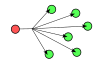
\includegraphics[width=0.3\linewidth]{Broadcast.png}
    \end{figure}

    \newpage
    \subparagraph{Anycast:} 
    One sender transmits to a group of other peers.
    \begin{figure}[h!]
        
\includegraphics[width=0.3\linewidth]{Anycast.png}
    \end{figure}

    \subparagraph{Geocast:} 
    Special form of multicast, one sender transmits to several receivers within a specific location.
    Uses coordinates in WGS84 as used in, for example, GPS.
    \begin{figure}[h!]
        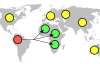
\includegraphics[width=0.3\linewidth]{Geocast.png}
    \end{figure}

\pagebreak

	\subsection{Cost efficient network upgrade}
	\paragraph{Given the network architecutre shown above, what is the maximum network throughput when all clients access random servers in parallel?}
	
	
	 Every computer gets 10 MBit/s in the standard configurarion. \newline
	 The bottleneck is the connection between a and b with 100 Mbit/s. We split this signal for the other two connections (b-c and b-d) to 50 MBit/s per connection. For every computer we split the signal again, resulting in 10 Mbit/s for each computer.\newline
The maximum throughput is at the bottleneck with 100MBit/s.  
	
	\begin{figure}[ht]
		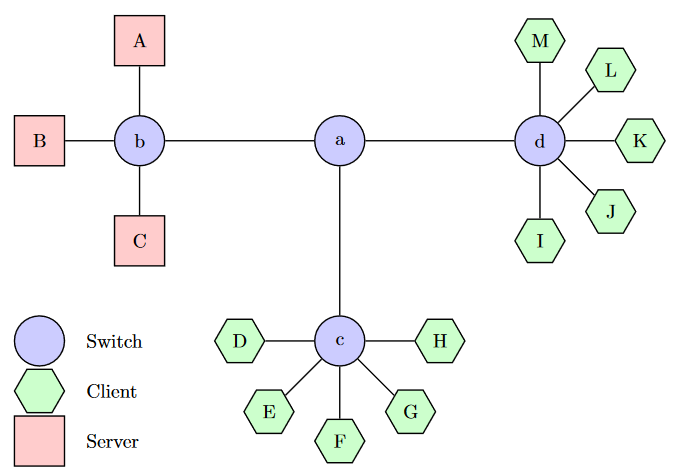
\includegraphics[width=0.7\linewidth]{network1.png}
		\caption{given network}
	\end{figure}


	\paragraph{You could upgrade the 100 MBit/s connections to 1 GBit/s.  However, you wonder if you could achieve a significant speed up with only upgrading a few connections. Show all intermediate steps to get higher network throughput until a full GBit/s network. How big are the speed ups?}	
	
	Solutions here: 
	\begin{table}[h!]
		%\caption{Upgradet Speed}
		\begin{minipage}{0.9\linewidth}
			\begin{tabular}{l|c|c|c|c|c} 
				\textbf{upgrade step} & \textbf{\mycirc{S}-b} & \textbf{b-a} & \textbf{a-c,a-d} & \textbf{\mycirc{C}-}c & \textbf{\mycirc{C}-d}		\\ \hline
				default & 100mb & 100mb & 50mb & 10mb & 10mb \\
				b+a & 100mb & 300mb & 100mb & 20mb & 20mb \\ 
				a+c,a+d & 100mb & 300mb & 150mb & 30mb & 30mb \\
				\mycirc{S}-b & 1gb & 1gb & 500mb & 100mb & 100mb \\
				all connections & 1gb & 1gb & 500mb & 100mb & 100mb \\ \hline
			\end{tabular} \\
			\footnotesize{$^{x-y}$ connection between x and y, $^{x+y}$ upgrade connection, $^S$ Server, $^C$ Clients}
		\end{minipage}
	\end{table}



\end{document}
